\section{Sharp codimension barriers and distributional stability}
\label{codim:section}

The Fourier-degree condition imposes useful restrictions on each cell
separately.  For the first three codimensions, these restrictions determine
the least possible conditional variance of the coordinate sum.  They also
give a quantitative description of every cell whose variance is close to
that minimum.  The description concerns a probability distribution:
different cells can have the same distribution of the coordinate sum
without having the same geometry.

\subsection{Alternating moments and two interlaced lattices}

\begin{lemma}[Alternating-moment cancellation]
\label{codim:alternating}
Let \(1\le k\le N\), let \(C\subseteq\{-1,1\}^N\) have positive
uniform probability, and suppose
\(\deg\1_C\le N-k\).  For
\[
Y=\frac{N-H_N}{2},
\]
one has
\begin{equation}
\label{codim:alternating-equation}
\E[(-1)^Y Y^j\mid C]=0
\qquad(0\le j<k).
\end{equation}
In particular, conditional on \(C\), the even and odd values of \(Y\)
each have probability \(1/2\).  Their normalized conditional
distributions have identical moments through order \(k-1\).
\end{lemma}

\begin{proof}
The variable \(Y\) counts the negative coordinates, so
\[
(-1)^Y=\chi_{[N]}(X).
\]
The function \(Y^j\), after multilinear reduction on the cube, has
Fourier degree at most \(j\).  Multiplication by \(\chi_{[N]}\)
takes \(\chi_S\) to \(\chi_{[N]\setminus S}\).  Thus
\(\chi_{[N]}Y^j\) has Fourier support only at degrees at least
\(N-j>N-k\).  Orthogonality of the Walsh characters gives
\[
\E[\1_C\chi_{[N]}Y^j]=0.
\]
Division by \(\Pbb(C)>0\) proves
\eqref{codim:alternating-equation}.

The equation for \(j=0\) gives parity balance.  For any subsequent
\(j\), the same equation says that the unnormalized \(j\)-th moments
on the two parity classes agree.  Since the classes each have mass
\(1/2\), their normalized moments agree as well.
\end{proof}

The following elementary fact supplies the needed variance estimates.
Its equality condition will be used repeatedly.

\begin{lemma}[Variance on a lattice of spacing two]
\label{codim:lattice}
Suppose \(Z\) takes values in \(a+2\Z\), has finite second moment,
and has mean \(\mu\in[a,a+2]\).  Then
\begin{equation}
\label{codim:lattice-bound}
\Var(Z)\ge(\mu-a)(a+2-\mu).
\end{equation}
Equality holds if and only if \(Z\) is supported on
\(\{a,a+2\}\).  In that case its probabilities are necessarily
\((a+2-\mu)/2\) and \((\mu-a)/2\).
\end{lemma}

\begin{proof}
For every \(z\in a+2\Z\), the product
\((z-a)(z-a-2)\) is nonnegative and vanishes exactly at \(a,a+2\).
Taking expectations and expanding gives
\[
0\le \E[(Z-a)(Z-a-2)]
=\Var(Z)-(\mu-a)(a+2-\mu).
\]
The equality statement follows from pointwise nonnegativity.
The mean determines the two probabilities.
\end{proof}

\begin{proposition}[The first three alternating-moment bounds]
\label{codim:moment-variance}
Let \(k\in\{1,2,3\}\), and let \(Y\) be integer valued with finite
second moment and
\begin{equation}
\label{codim:abstract-moments}
\E[(-1)^Y Y^j]=0
\qquad(0\le j<k).
\end{equation}
Then
\[
\Var(Y)\ge k/4.
\]
Equality holds if and only if
\[
\Law(Y)=\Law(m+B_k)
\]
for some integer \(m\), where \(B_k\) has distribution
\(\operatorname{Bin}(k,1/2)\).
\end{proposition}

\begin{proof}
Translation by an integer preserves
\eqref{codim:abstract-moments}: the parity factor changes by a constant
sign, and a translated \(j\)-th power is a polynomial of degree at most
\(j\).  We can therefore translate the mean to an interval convenient
for the proof.

For \(k=1\), translate so that \(\mu=\E Y\in[0,1]\).  Each parity
has mass \(1/2\).  The nearest even lattice point to \(\mu\) is \(0\),
and the nearest odd lattice point is \(1\), with a possible tie at an
endpoint.  Hence
\[
\Var(Y)
\ge \frac12\mu^2+\frac12(1-\mu)^2
=\frac14+(\mu-1/2)^2.
\]
Equality at \(1/4\) forces \(\mu=1/2\), and then forces the even
and odd conditional laws to be point masses at \(0\) and \(1\).
This is \(B_1\).

For \(k\ge2\), the conditional means on the two parity classes
agree.  Write their common mean as \(\mu\), and translate it to
\(u\in[0,1]\).  The even and odd conditional variances, denoted by
\(V_e,V_o\), satisfy
\begin{equation}
\label{codim:AB}
V_e\ge A(u):=u(2-u),
\qquad
V_o\ge B(u):=1-u^2,
\end{equation}
by Lemma~\ref{codim:lattice}, using the pairs \(\{0,2\}\) and
\(\{-1,1\}\), respectively.

For \(k=2\), the equality of conditional means gives
\[
\Var(Y)=\frac{V_e+V_o}{2}
\ge\frac12+u-u^2
\ge\frac12.
\]
Equality requires \(u=0\) or \(u=1\), together with equality in
both lattice bounds.  At \(u=0\), the even law is the point mass at
\(0\), and the odd law has equal masses at \(-1,1\).
The full law has weights \((1,2,1)/4\) on \(-1,0,1\).
The case \(u=1\) is its integer translate.  These are precisely
the translates of \(B_2\).

For \(k=3\), the conditional second moments agree in addition to
the means, so
\[
V_e=V_o=\Var(Y).
\]
Consequently
\[
\Var(Y)\ge\max\{A(u),B(u)\}
=\frac34+|u-1/2|-|u-1/2|^2
\ge\frac34.
\]
Since \(|u-1/2|\le1/2\), equality at \(3/4\) forces \(u=1/2\).
Equality in both instances of Lemma~\ref{codim:lattice} then gives
the full probabilities
\[
\frac18,\quad\frac38,\quad\frac38,\quad\frac18
\]
on \(-1,0,1,2\), which is \(B_3-1\).

Conversely, every translate of \(B_k\) has variance \(k/4\)
and satisfies the required cancellations.  For the latter assertion,
\[
\E[(-1)^{B_k}z^{B_k}]=2^{-k}(1-z)^k;
\]
applying \((z\,d/dz)^j\) and evaluating at \(z=1\) gives zero for
\(j<k\).  Integer translation preserves these cancellations.
\end{proof}

\begin{theorem}[Cellwise variance barrier]
\label{codim:barrier}
Let \(k\in\{1,2,3\}\), let \(N\ge k\), and suppose
\(D(F)\le N-k\).  Every attained cell \(C=\{F=a\}\) satisfies
\begin{equation}
\label{codim:cell-barrier}
\Var(H_N\mid F=a)\ge k.
\end{equation}
Therefore
\begin{equation}
\label{codim:retained-barrier}
v(F)\le N-k.
\end{equation}
Equality in \eqref{codim:cell-barrier} holds exactly when the
conditional law of \(H_N\) is an integer translate of the sum of
\(k\) independent uniform signs.  Equality in
\eqref{codim:retained-barrier} holds exactly when this condition holds
in every attained cell, with a possibly different translate in each
cell.  Revealing any \(N-k\) coordinates attains equality.
\end{theorem}

\begin{proof}
Lemma~\ref{codim:alternating} and
Proposition~\ref{codim:moment-variance} apply to
\(Y=(N-H_N)/2\) in each cell.  Since
\(\Var(H_N\mid C)=4\Var(Y\mid C)\), they prove the cellwise
bound and its equality characterization.  More explicitly, if
\(Y\mid C\) has law \(m+B_k\), then
\[
H_N\mid C\ \stackrel{\rm law}{=}\
N-2m-k+S_k,
\]
where \(S_k=k-2B_k\) is a sum of \(k\) uniform signs.
The translate consequently has the parity required by the original
cube.

The total variance identity gives
\[
N=\Var(H_N)
=v(F)+\E[\Var(H_N\mid F)].
\]
A finite positive-weight average of quantities each at least \(k\)
equals \(k\) if and only if every quantity equals \(k\).  This proves
the retained-variance statement and its equality condition.
Finally, after \(N-k\) coordinates are revealed, the remaining
\(k\) signs are independent and uniform.  The cell indicators have
degree \(N-k\), and the conditional variance is exactly \(k\).
\end{proof}

\begin{corollary}[Bounds that retain the conditional mean]
\label{codim:mean-sensitive}
Let \(C\) be a cell as in Lemma~\ref{codim:alternating}, and let
\(u\in[0,1]\) be the fractional part of
\(\E[(N-H_N)/2\mid C]\).  For \(k=2\),
\begin{equation}
\label{codim:mean-two}
\Var(H_N\mid C)\ge2+4u(1-u).
\end{equation}
For \(k=3\),
\begin{equation}
\label{codim:mean-three}
\Var(H_N\mid C)
\ge3+4|u-1/2|-4|u-1/2|^2.
\end{equation}
\end{corollary}

\begin{proof}
These are the two estimates before minimization over \(u\) in the
proof of Proposition~\ref{codim:moment-variance}, multiplied by four.
\end{proof}

\begin{figure}[tb]
\centering
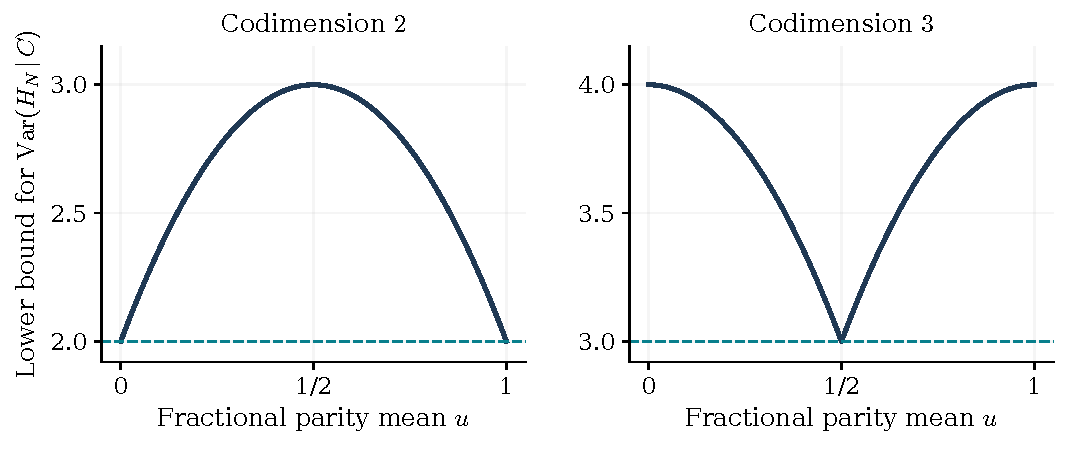
\includegraphics[width=.94\linewidth]{figures/parity_bounds.pdf}
\caption{The mean-sensitive conditional-variance bounds. The fractional
part \(u\) of the common parity-conditioned Hamming-weight mean
controls the extra variance forced by the two interlacing lattices.
Dashed lines mark the universal minima.}
\label{fig:parity-bounds}
\end{figure}

\begin{remark}
All the preceding assertions hold for a signed coordinate sum
\(\sum_i\epsilon_iX_i\), with fixed \(\epsilon_i\in\{-1,1\}\).
The change of variables \(X_i\mapsto\epsilon_iX_i\) preserves the
uniform law and every Fourier degree.  The equality statements
classify the conditional laws of these sums; they do not characterize
which coordinates a cell fixes.
\end{remark}

\subsection{A stable projection onto neighboring lattice points}

We use the convention
\[
\TV(P,Q)=\frac12\sum_{z\in\Z}|P\{z\}-Q\{z\}|.
\]
Here and below, \(\delta_z\) denotes a unit point mass at \(z\).
The next estimate controls the entire distribution by the slack in
Lemma~\ref{codim:lattice}.

\begin{lemma}[Stable lattice projection]
\label{stab:lattice-projection}
Under the hypotheses of Lemma~\ref{codim:lattice}, set
\[
Q_\mu=\frac{a+2-\mu}{2}\delta_a+
      \frac{\mu-a}{2}\delta_{a+2}.
\]
Then
\begin{equation}
\label{stab:projection-bound}
\TV(\Law(Z),Q_\mu)
\le\frac14\left\{
\Var(Z)-(\mu-a)(a+2-\mu)
\right\}.
\end{equation}
Moreover,
\begin{equation}
\label{stab:outside-bound}
\Pbb\{Z\notin\{a,a+2\}\}
\le\frac18\left\{
\Var(Z)-(\mu-a)(a+2-\mu)
\right\}.
\end{equation}
\end{lemma}

\begin{proof}
Put \(J=(Z-a)/2\) and \(t=\E J\in[0,1]\).  The slack, divided
by four, is
\[
S=\E[J(J-1)]\ge0.
\]
Let
\[
q=\Pbb\{J\notin\{0,1\}\},
\qquad
b=\E[J\1_{\{J\notin\{0,1\}\}}].
\]
The differences between the actual masses at \(0,1\) and the target
masses \(1-t,t\) are \(b-q,-b\), respectively.  Therefore
\[
\TV\bigl(\Law(J),(1-t)\delta_0+t\delta_1\bigr)
=\frac{q+|b-q|+|b|}{2}
=\max\{q,b,q-b\}.
\]
For every integer \(j\notin\{0,1\}\),
\[
1\le j(j-1),\qquad
j\le j(j-1),\qquad
1-j\le j(j-1).
\]
Their expectations give \(q,b,q-b\le S\), proving
\eqref{stab:projection-bound}.  Finally,
\(j(j-1)\ge2\) outside \(\{0,1\}\), so \(q\le S/2\).
This proves \eqref{stab:outside-bound}.
\end{proof}

\subsection{Quantitative stability near the three variance minima}

\begin{definition}
\label{stab:distance-definition}
For an integer-valued random variable \(Y\), define its distance from
the binomial translates by
\[
d_k(Y)=\inf_{m\in\Z}
\TV\bigl(\Law(Y),\Law(m+B_k)\bigr),
\qquad B_k\sim\operatorname{Bin}(k,1/2).
\]
For \(0\le\delta\le1/4\), write
\[
r(\delta)=\frac{1-\sqrt{1-4\delta}}2.
\]
Thus \(0\le r(\delta)\le1/2\) and
\(r(\delta)-r(\delta)^2=\delta\).
\end{definition}

\begin{theorem}[Linear stability, with explicit local moduli]
\label{stab:main}
Let \(Y\) satisfy the assumptions of
Proposition~\ref{codim:moment-variance}, and put
\(\delta=\Var(Y)-k/4\ge0\).  For \(k=1,2\),
\begin{equation}
\label{stab:global-twelve}
d_k(Y)\le\delta.
\end{equation}
For \(k=3\),
\begin{equation}
\label{stab:global-three}
d_3(Y)\le\frac32\delta.
\end{equation}
When \(0\le\delta\le1/4\), the stronger bounds are
\begin{align}
d_k(Y)&\le\frac12r(\delta)
=\frac{1-\sqrt{1-4\delta}}4,
&& k=1,2,
\label{stab:local-twelve}\\
d_3(Y)&\le\frac34r(\delta)
=\frac38\bigl(1-\sqrt{1-4\delta}\bigr).
\label{stab:local-three}
\end{align}
In particular,
\begin{equation}
\label{stab:small-three}
d_3(Y)\le\delta
\qquad(0\le\delta\le3/16).
\end{equation}
Every bound is obtained by an explicitly chosen integer translate.
\end{theorem}

\begin{proof}
Integer translation and reflection preserve the alternating-moment
conditions.  They also preserve \(d_k\), since \(k-B_k\) and \(B_k\)
have the same law.  We use these operations to normalize the mean.

\paragraph{The case \(k=1\).}
Translate so that \(u=\E Y\in[0,1]\), and put
\(a=|u-1/2|\le1/2\).  Then
\[
S:=\E[Y(Y-1)]
=\Var(Y)+u^2-u
=\delta+a^2.
\]
Let \(b(y)\) be \(0\) or \(1\) according to the parity of the
integer \(y\).  Parity balance gives \(\E b(Y)=1/2\).
For every integer \(y\),
\[
|y-b(y)|\le y(y-1).
\]
For \(y=0,1\) both sides vanish; for all other integers the
inequality follows immediately by considering \(y\le-1\) and
\(y\ge2\).  Consequently
\[
a=|\E[Y-b(Y)]|\le S,
\qquad
\delta\ge a-a^2.
\]
Every single atom of \(Y\) has mass at most \(1/2\).  Thus its
distance from \((\delta_0+\delta_1)/2\) is exactly
\(q=\Pbb\{Y\notin\{0,1\}\}\).
Since \(y(y-1)\ge2\) outside those two integers,
\begin{equation}
\label{stab:one-intermediate}
d_1(Y)\le q\le\frac{\delta+a^2}{2}.
\end{equation}
Because \(a\le1/2\), we have
\(\delta\ge a-a^2\ge a^2\), which proves
\eqref{stab:global-twelve} for \(k=1\).
If \(\delta\le1/4\), the monotonicity of \(x-x^2\) on
\([0,1/2]\) gives \(a\le r(\delta)\).  Substituting this in
\eqref{stab:one-intermediate} and using
\(\delta+r(\delta)^2=r(\delta)\) proves
\eqref{stab:local-twelve}.

\paragraph{Common notation for \(k=2,3\).}
The parity-conditioned means agree.  After translation, suppose their
common value is \(u\in[0,1]\), and define
\[
Q_e^u=(1-u/2)\delta_0+(u/2)\delta_2,
\qquad
Q_o^u=((1-u)/2)\delta_{-1}+((1+u)/2)\delta_1.
\]
Their variances are \(A(u),B(u)\) from \eqref{codim:AB}.
Their equally weighted mixture is
\begin{equation}
\label{stab:nu}
\nu_u=
\frac{1-u}{4}\delta_{-1}
+\frac{2-u}{4}\delta_0
+\frac{1+u}{4}\delta_1
+\frac{u}{4}\delta_2.
\end{equation}
The even and odd supports are disjoint, so
Lemma~\ref{stab:lattice-projection} gives
\begin{equation}
\label{stab:mixture-projection}
\TV(\Law(Y),\nu_u)
\le\frac{V_e-A(u)+V_o-B(u)}8.
\end{equation}

\paragraph{The case \(k=2\).}
Choose the nearest integer to the common mean, translate to that
integer, and reflect if necessary.  We then have \(u\in[0,1/2]\).
Since
\(\Var(Y)=(V_e+V_o)/2=1/2+\delta\), the two nonnegative
lattice slacks yield
\[
\delta\ge u-u^2,
\qquad
\TV(\Law(Y),\nu_u)
\le\frac{\delta-u+u^2}{4}.
\]
The law \(\nu_0\) is that of \(B_2-1\).
Direct comparison in \eqref{stab:nu} gives
\(\TV(\nu_u,\nu_0)=u/2\).  Hence
\begin{equation}
\label{stab:two-intermediate}
d_2(Y)\le\frac{\delta+u+u^2}{4}.
\end{equation}
For \(0\le u\le1/2\),
\[
u+u^2\le3(u-u^2)\le3\delta,
\]
which proves the global bound.  If \(\delta\le1/4\),
then \(u\le r(\delta)\), and
\eqref{stab:two-intermediate} becomes
\[
d_2(Y)\le\frac{\delta+r(\delta)+r(\delta)^2}{4}
=\frac12r(\delta).
\]

\paragraph{The case \(k=3\).}
Translate the common parity mean to \(u\in[0,1]\), and put
\(a=|u-1/2|\).  Here
\(V_e=V_o=3/4+\delta\), and \eqref{codim:AB} gives
\[
\delta\ge a-a^2.
\]
Since \(A(u)+B(u)=3/2-2a^2\),
\eqref{stab:mixture-projection} reads
\[
\TV(\Law(Y),\nu_u)\le\frac{\delta+a^2}{4}.
\]
The law \(\nu_{1/2}\) is that of \(B_3-1\), and
\(\TV(\nu_u,\nu_{1/2})=a/2\).  We obtain
\begin{equation}
\label{stab:three-intermediate}
d_3(Y)\le\frac{\delta+a^2+2a}{4}.
\end{equation}
For \(a\in[0,1/2]\),
\[
a^2+2a\le5(a-a^2)\le5\delta,
\]
proving \eqref{stab:global-three}.
When \(\delta\le1/4\), we have \(a\le r(\delta)\), and
\eqref{stab:three-intermediate} gives
\[
d_3(Y)\le
\frac{\delta+r(\delta)^2+2r(\delta)}4
=\frac34r(\delta).
\]
Finally, if \(\delta\le3/16\), then \(a\le r(\delta)\le1/4\),
and the stronger inequality
\[
a^2+2a\le3(a-a^2)\le3\delta
\]
in \eqref{stab:three-intermediate} proves
\eqref{stab:small-three}.
\end{proof}

\subsection{Sharpness in the alternating-moment class}

We record exact families attaining the local estimates.  Their role is
to identify the best possible modulus under the stated moment
conditions.  An additional realization argument would be needed to
assert the same optimality among uniform laws on Fourier-degree
constrained cube cells.

\begin{proposition}[Sharp local moduli]
\label{stab:sharpness}
The bounds \eqref{stab:local-twelve} are attained for every
\(0\le\delta\le1/4\).  The bound \eqref{stab:local-three} is
attained for every \(0\le\delta\le3/16\).  Thus the leading constants
\(1/2,1/2,3/4\) in front of \(\delta\) are optimal in the
alternating-moment class for \(k=1,2,3\), respectively.
\end{proposition}

\begin{proof}
First note a separation fact.  Any two distinct integer translates
of \(B_k\) are at TV distance at least its largest atom.  Indeed,
let \(j_*\) be a largest atom, and compare \(B_k\) with \(B_k+h\),
where \(h\ge1\).  On the event \((-\infty,j_*]\), the difference
of their probabilities is
\[
\Pbb\{j_*-h<B_k\le j_*\}\ge\Pbb\{B_k=j_*\}.
\]
Negative shifts are reduced to positive ones by translation and
symmetry of TV.  The largest atom equals \(1/2\) for \(k=1,2\)
and \(3/8\) for \(k=3\).  Consequently, whenever a law is at
distance at most half this separation from one translate, no other
translate can be closer: this follows from the triangle inequality.

For \(k=1\), let \(0\le t\le1/2\), and take
\[
\Pbb\{Y=0\}=(1-t)/2,\qquad
\Pbb\{Y=1\}=1/2,\qquad
\Pbb\{Y=2\}=t/2.
\]
Parity balance holds.  The mean and second moment are
\(1/2+t\) and \(1/2+2t\), so
\[
\Var(Y)=1/4+t-t^2.
\]
Its distance from \(B_1\) is \(t/2\le1/4\), making \(B_1\)
a nearest translate by the separation fact.

For \(k=2\), take \(Y\) with law \(\nu_t\) from
\eqref{stab:nu}, again with \(0\le t\le1/2\).
Each parity has mass \(1/2\), and both conditional means are \(t\).
The second moment is \(1/2+t\), whence
\[
\Var(Y)=1/2+t-t^2.
\]
Its distance from \(B_2-1=\nu_0\) is \(t/2\le1/4\).
This translate is therefore nearest.

For \(k=3\), let \(0\le t\le1/4\), and use the five-point law
\begin{equation}
\label{stab:sharp-three-family}
\begin{array}{c|ccccc}
y&-3&-1&0&1&2\\ \hline
\Pbb\{Y=y\}
&t/8&1/8-t/2&3/8-t/4&3/8+3t/8&1/8+t/4 .
\end{array}
\end{equation}
All its probabilities are nonnegative and sum to one.  The even
and odd classes each have mass \(1/2\).  Their normalized first
moments both equal \(1/2+t\), and their normalized second moments
both equal \(1+2t\).  Thus all three required alternating moments
vanish, and
\[
\Var(Y)=1+2t-(1/2+t)^2=3/4+t-t^2.
\]
Relative to \(B_3-1\), the positive mass differences occur at
\(-3,1,2\), and sum to
\[
t/8+3t/8+t/4=3t/4.
\]
This is at most \(3/16\), so the displayed binomial translate is
nearest.

In all three families, \(\delta=t-t^2\), hence
\(t=r(\delta)\).  The first two parameter intervals cover
\(\delta\in[0,1/4]\); the third covers \(\delta\in[0,3/16]\).
These are exactly the stated attainment ranges.
Finally \(r(\delta)=\delta+O(\delta^2)\) as
\(\delta\downarrow0\), which proves the assertion about leading
constants.
\end{proof}

\subsection{From cellwise stability to the joint observation law}

\begin{corollary}[Stability in the coordinate-sum normalization]
\label{stab:cell}
Under the cell hypotheses of Theorem~\ref{codim:barrier}, suppose
\[
\Var(H_N\mid C)\le k+\varepsilon
\]
for some \(\varepsilon\ge0\).
There is an integer \(c\equiv N-k\pmod2\) such that
\[
\TV\bigl(\Law(H_N\mid C),\Law(c+S_k)\bigr)
\le
\begin{cases}
\varepsilon/4,&k=1,2,\\
3\varepsilon/8,&k=3.
\end{cases}
\]
If \(0\le\varepsilon\le1\), the respective stronger bounds are
\[
\frac{1-\sqrt{1-\varepsilon}}4
\quad(k=1,2),
\qquad
\frac38\bigl(1-\sqrt{1-\varepsilon}\bigr)
\quad(k=3).
\]
For \(k=3\) and \(\varepsilon\le3/4\), the bound
\(\varepsilon/4\) is valid as well.
\end{corollary}

\begin{proof}
Apply Theorem~\ref{stab:main} to the conditional law of
\(Y=(N-H_N)/2\), for which
\[
0\le\delta=\Var(Y\mid C)-k/4\le\varepsilon/4.
\]
All the displayed bounding functions are increasing on their stated
domains.  TV is unchanged under the bijection \(y\mapsto N-2y\)
from \(\Z\) onto the parity lattice \(N+2\Z\).
The binomial translate \(m+B_k\) is sent to
\(c+S_k\), where \(c=N-2m-k\).  This also proves the parity
assertion.
\end{proof}

\begin{corollary}[Joint-law stability near saturation]
\label{stab:joint}
Let \(k\in\{1,2,3\}\), suppose \(D(F)\le N-k\), and put
\[
\Delta=(N-k)-v(F)\ge0.
\]
There is an integer-valued function \(c\) of the attained labels of
\(F\), with \(c(a)\equiv N-k\pmod2\), such that
\begin{equation}
\label{stab:joint-bound}
\TV\bigl(\Law(F,H_N),\Law(F,c(F)+S_k)\bigr)
\le C_k\Delta,
\qquad
C_1=C_2=\frac14,\quad C_3=\frac38,
\end{equation}
where \(S_k\) is independent of \(F\).
For \(k=3\), one may replace \(C_3\) by \(1/4\) if every attained
cell satisfies
\(\Var(H_N\mid F=a)\le3+3/4\).
\end{corollary}

\begin{proof}
For each attained label \(a\), let
\[
\varepsilon_a=\Var(H_N\mid F=a)-k\ge0
\]
and choose \(c(a)\) by Corollary~\ref{stab:cell}.  The observation
has finitely many attained labels, so this defines the desired function
without a selection issue.  Construct the comparison law using the
same \(F\)-marginal and an independent \(S_k\).
For two joint laws with the same first marginal, direct summation of
the absolute differences gives
\begin{align*}
&\TV\bigl(\Law(F,H_N),\Law(F,c(F)+S_k)\bigr)\\
&\qquad=
\sum_a\Pbb\{F=a\}
\TV\bigl(\Law(H_N\mid F=a),\Law(c(a)+S_k)\bigr)\\
&\qquad\le C_k\sum_a\Pbb\{F=a\}\varepsilon_a.
\end{align*}
The last sum is
\[
\E[\Var(H_N\mid F)]-k
=N-v(F)-k=\Delta.
\]
This proves \eqref{stab:joint-bound}.  The additional cellwise
hypothesis permits the improved constant in
Corollary~\ref{stab:cell} for every summand.
\end{proof}

\begin{remark}
The model in \eqref{stab:joint-bound} is a mixture of translated
\(k\)-sign sums with a quantitatively controlled error.  Applying the
projection \((a,h)\mapsto h\) gives the same bound for the
unconditional coordinate-sum marginals.  Neither conclusion asserts
that the observation is close to a coordinate-revealing map or that
its cells are close to subcubes.  Controlling such geometric features
would require additional information beyond the law of the sum.
\end{remark}

\subsection{The fourth-order moment relaxation}

The alternating-moment condition alone changes character at the next
order.  The following proposition concerns an abstract moment class;
it supplies no construction of a cube cell.

\begin{proposition}[The order-four relaxation]
\label{codim:four-relaxation}
Among integer-valued laws with finite third absolute moment satisfying
\[
\E[(-1)^Y Y^j]=0\qquad(0\le j\le3),
\]
the infimum of \(\Var(Y)\) is \(3/4\), and the infimum is not
attained.  In particular, fourth-order cancellation does not imply
\(\Var(Y)\ge1\).
\end{proposition}

\begin{proof}
The lower bound \(3/4\) follows from
Proposition~\ref{codim:moment-variance} with \(k=3\).
To approach it while retaining the fourth cancellation, let
\(R\ge5\) be an integer with \(R\equiv1\pmod4\), and define
\[
a_R=\frac{6}{(R-1)(R+3)(R-2)},\qquad
c_R=\frac{R(R^2-1)}{24}\,a_R,\qquad
b_R=3c_R-Ra_R.
\]
All three weights are positive.  Indeed,
\[
b_R=\frac{R(R^2-9)}8\,a_R>0.
\]
Furthermore,
\[
a_R+b_R+c_R
=a_R\frac{R^3-7R+6}{6}=1,
\]
because \(R^3-7R+6=(R-1)(R+3)(R-2)\).
Let \(Z_R\) have probabilities \(a_R,b_R,c_R\) at
\(-R,-1,3\), respectively.  These three points lie in \(4\Z-1\).
The definitions give
\[
\E Z_R=-Ra_R-b_R+3c_R=0,
\]
and
\[
\E Z_R^3
=-R^3a_R-b_R+27c_R
=-R(R^2-1)a_R+24c_R=0.
\]
The second moment is
\[
\E Z_R^2
=R^2a_R+b_R+9c_R
=\frac{R(R-1)(R+3)}2a_R
=\frac{3R}{R-2}.
\]

Let \(W_R\) have the equally weighted mixture of the laws of
\(Z_R\) and \(-Z_R\), and put \(Y_R=(W_R+1)/2\).
The two components of \(W_R\) lie in the distinct cosets
\(4\Z-1\) and \(4\Z+1\).  They have matching moments of orders
zero through three: their odd moments of orders one and three are
zero, and their even moments agree by reflection.
After the affine change to \(Y_R\), these are the two parity classes.
Therefore
\[
\E[(-1)^{Y_R}Y_R^j]=0\qquad(0\le j\le3),
\]
while
\[
\Var(Y_R)=\frac{3R}{4(R-2)}\longrightarrow\frac34.
\]
For example, \(R=9\) gives the exact law
\[
\begin{array}{c|rrrrrr}
y&-4&-1&0&1&2&5\\ \hline
224\,\Pbb\{Y_R=y\}&1&30&81&81&30&1
\end{array}
\]
with variance \(27/28<1\).

Finally, if a law satisfying all four cancellations attained variance
\(3/4\), Proposition~\ref{codim:moment-variance} would make it
a translate \(m+B_3\).  But
\[
\E[(-1)^{m+B_3}(m+B_3)^3]
=(-1)^m\E[(-1)^{B_3}B_3^3]
=(-1)^{m+1}\frac34\ne0.
\]
Here the lower-order terms vanish by the first three cancellations
for \(B_3\).  This contradicts the fourth one and proves
nonattainment.
\end{proof}

